%!TEX root = ../../../main.tex

\subsection{MuHAVi dataset}
    The MuHAVi dataset is constructed and introduced by \cite{murtaza2016multi}. It is usually referred as MuHAVi-uncut because it contains full, raw videos of 17 actions, asynchronously captured by eight cameras that provide completely overlapping coverage of a rectangular action zone from different viewing directions as in Fig.\ref{Fig:MuHAVi1}. 

    \begin{figure}[h]
        \centering
        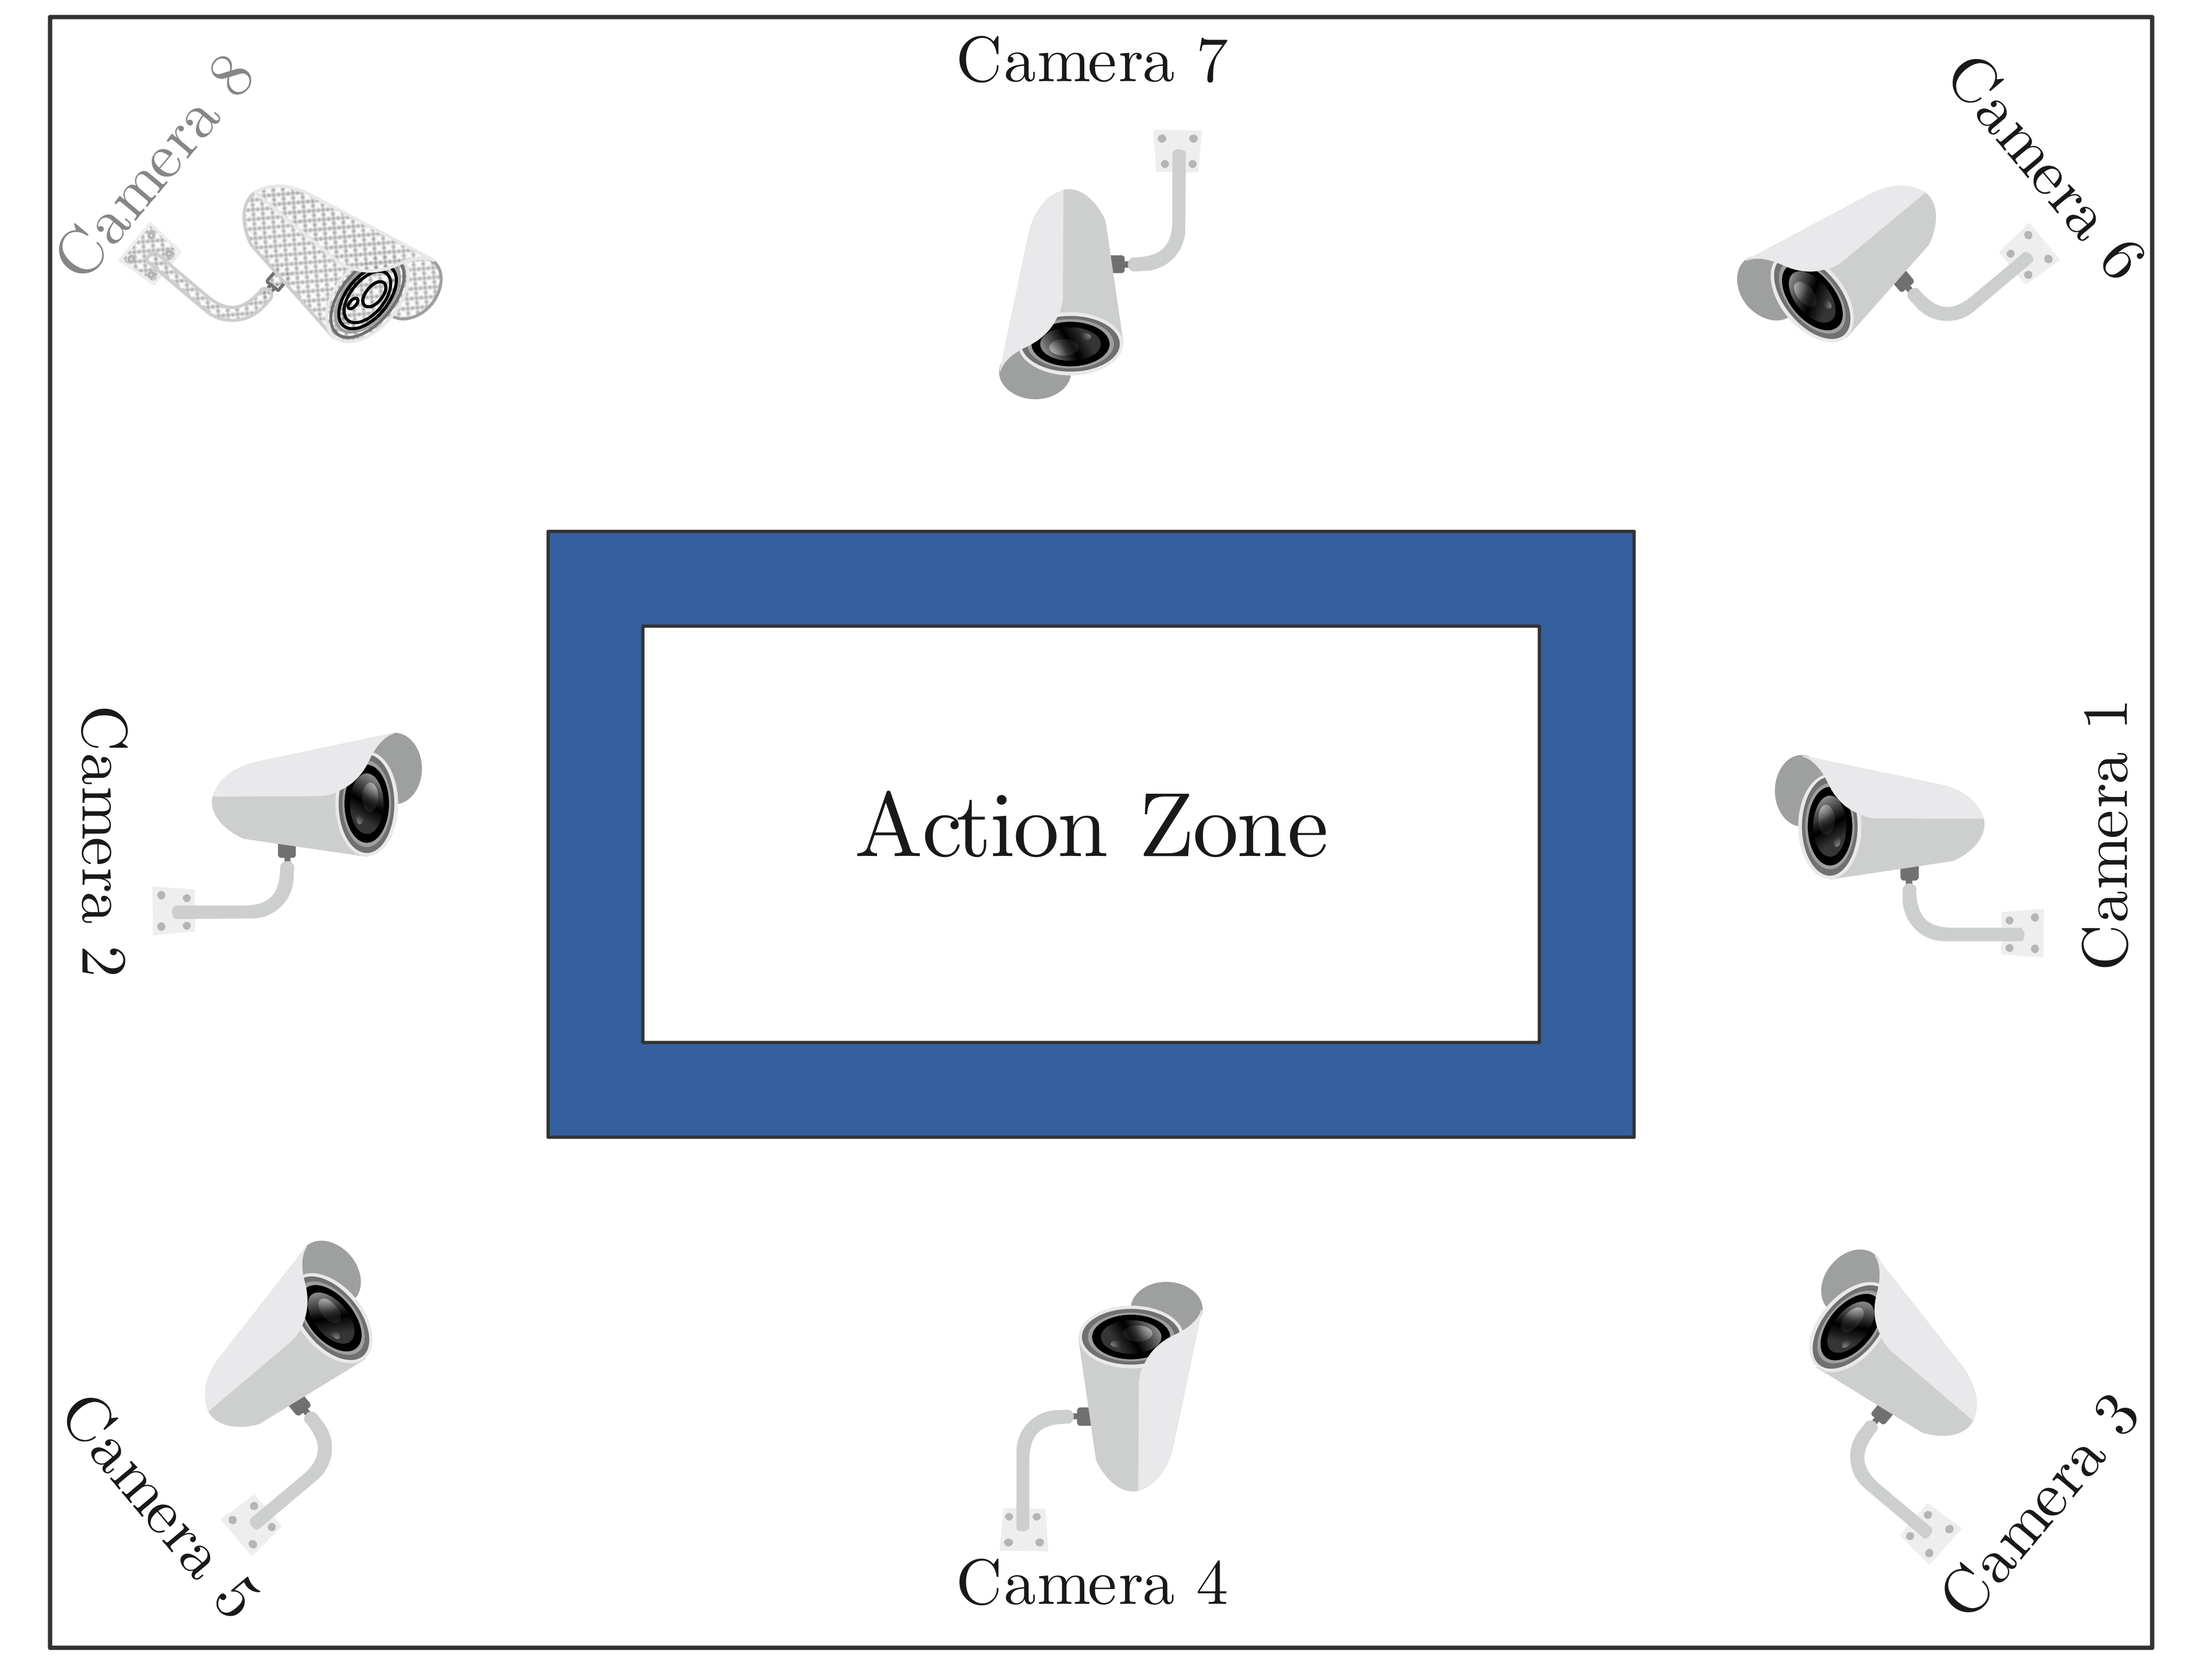
\includegraphics[width=0.8\linewidth]{figs/MuHAVi1.png}
        \caption{Environment setup to collect action sequences from 8 views \cite{murtaza2016multi}.}
        %\vspace{-0.3cm}
        \label{Fig:MuHAVi1}
    \end{figure}

    The actions are are walk turn back, run stop, punch, kick, shotgun collapse, pull heavy object, pickup throw object, walk fall, look in car, crawl on knees, wave arms, draw graffiti, jump over fence, drunk walk, climb ladder, smash object, and jump over gap. 
    Each was performed several times by 7 actors (5 males / 2 females). 
    The videos were collected at rate of 25 fps with resolution of 720 $\times$ 576, except for the $8^{th}$ camera whose data is not included in experiments of this thesis due to absence of annotation.
    Some representative frames of action \textit{punch} are shown in Fig.\ref{Fig:MuHAVi2}.

    \begin{figure}[htbp]
        \centering
        \includegraphics[width=1\linewidth]{figs/MuHAVi2.png}
        \caption{Illustration of frames extracted from an action \textit{punch} observed from Camera 1 to Camera 7.}
        %\vspace{-0.3cm}
        \label{Fig:MuHAVi2}
    \end{figure}
